\documentclass[compsoc]{IEEEtran}

%\usepackage{cite}
\ifCLASSINFOpdf
  \usepackage[pdftex]{graphicx}
\else
  \usepackage[dvips]{graphicx}
\fi
\usepackage[cmex10]{amsmath}
\usepackage{stfloats}

\ifCLASSOPTIONcaptionsoff
  \usepackage[nomarkers]{endfloat}
 \let\MYoriglatexcaption\caption
 \renewcommand{\caption}[2][\relax]{\MYoriglatexcaption[#2]{#2}}
\fi

\usepackage{url}
\usepackage{caption} % http://ctan.org/pkg/caption
\usepackage{booktabs}
\usepackage{enumitem}
\usepackage{listings}

\usepackage[style=ieee]{biblatex}

\addbibresource{references.bib} %Imports bibliography file

\begin{document}

\markboth{Chimakurthi, Han, Jain, Yang}{Business Dynamics and Neighborhood Characteristics}

\title{Understand Local Business Dynamics and \\
Neighborhood Characteristics with Yelp Data} % title

\author{Lakshmimanaswitha Chimakurthi, Zexi Han, Anant Jain, Jianchao Yang}

% As a general rule, do not put math, special symbols or citations
% in the abstract or keywords.
\IEEEtitleabstractindextext{%
\begin{abstract}
With comprehensive metadata about local businesses and user-generated contents such as reviews, check-ins and tips, the Yelp data contain copious information about local business dynamics. Using a variety of data mining techniques, including K-Means, PCA, GMM, and weighted feature scaling, we clustered neighborhoods based on the business dynamics shown in the Yelp data and neighborhood characteristics represented by census data, then explored the relationship between the two by evaluating the goodness of the clusters.
\end{abstract}}

% make the title area
\maketitle

% To allow for easy dual compilation without having to reenter the
% abstract/keywords data, the \IEEEtitleabstractindextext text will
% not be used in maketitle, but will appear (i.e., to be "transported")
% here as \IEEEdisplaynontitleabstractindextext when the compsoc 
% or transmag modes are not selected <OR> if conference mode is selected 
% - because all conference papers position the abstract like regular
% papers do.
\IEEEdisplaynontitleabstractindextext
% \IEEEdisplaynontitleabstractindextext has no effect when using
% compsoc or transmag under a non-conference mode.

\section{Introduction}

With a public contest called Yelp Data Challenge hosted every year, the Yelp dataset has been studied extensively. Previous studies include predicting star ratings of businesses  \cite{kongpredicting}, sentiment analysis and topic extraction for user reviews \cite{huang2014improving}, the efficiency of social networks \cite{wong2016efficiency}, etc. Most of the researches used only the Yelp dataset and focused on developing novel algorithms to extract a single piece of information; few have tried to interpret underlying data insights in a social context.

The local business dynamics shown in the Yelp data---popularity of a business, the concentration of different types businesses, behavioral patterns of patrons---are good indicators of the healthiness of local business landscape and how neighborhoods are shaped by businesses.

Studies have found that access to certain businesses have a strong impact on neighborhood characteristics or even the health and wellbeing of the residents \cite{morland2002neighborhood}.

By extracting census tract and neighborhood level measurements from Yelp data, and applying clustering algorithms on them, we set apart neighborhoods by their business dynamics. We then used social econometrics and demographic information obtained from census data to evaluate how neighborhood characteristics are associated with business dynamics.


\section{The Datasets}

\subsection{The Yelp Data}

The Yelp Dataset 2017 includes information for more than 156,000 businesses in 12 metropolitan areas across 4 countries. It has over 4,700,000 reviews, 200,000 pictures, 1,000,000 tips contributed by 1,100,000 users. \footnote{\url{https://www.yelp.com/dataset/challenge}} There is also a table for aggregated average hourly check-in counts for each business on each day of a week.

The metadata for businesses is comprehensive. There are attributes such as address, geo-coordinates, hours, price range and availability of certain amenities, including parking, credit card as a payment option, restaurant delivery.

\subsection{The Census Data}

We rely on census data to describe neighborhood characteristics. For simplicity, we limit our work to U.S. cities only. This allows us to use a single API endpoint to collect all the demographic and socioeconomic data we need.

 \url{Census.gov} provides a convenient API to download census data, and \url{Socialexplorer.com} offers an easy-to-navigate documentation of the census variables.
 
Most of the census variables are proportions of residents being of a certain population group, determined by sex, age, race, poverty status, and health insurance coverage, etc. There are also socioeconomic variables such as median house income, property value, and housing cost. See appendix for the full list of census variables.

\subsection{Geographic Boundaries}

In order to aggregate at the neighborhood levels, we would need to know which neighborhood a business is located in. The Yelp dataset has a ``neighborhood'' field, but the data is incomplete and inconsistent (only about 40\% of the businesses have this value set).

We would also need a clear definition of what a neighborhood is---many big cities often have more than one definitions, either by different agencies or at different times. We use Zillow Neighborhood Boundaries, a consolidated database for the neighborhood boundaries of all major U.S. cities, as our main reference for neighborhood delineation.

However, the Census Bureau does not publish census data according to  Zillow Neighborhood Boundaries. The geographic unit with readily available census data and closest to a conventional ``neighborhood'' is either \textit{Census Tract} or \textit{ZIP Code Tabulation Area}.  %It is theoretically possible to estimate for Zillow neighborhoods by examining their overlap of the census tracts, but that requires significant amount of work that is beyond the purview of this class. 

In this paper, we run aggregations at both the Zillow Neighborhood and Census Tract level. The former is for grouping neighborhoods based on the traditional definition of common folks, the latter is for the ease of comparing clustering with different data sources: Yelp data and the census data.

\section{Data Preparation}

\subsection{Data Reduction}

The Yelp dataset has businesses from 1,010 cities (including duplicates due to spelling inconsistencies). We decided to work only on U.S. cities. We then further reduced the dataset to contain businesses from only the top eight states with most businesses. This is because, by the ninth state, the number of businesses has dropped to a negligible level (Table \ref{top-states}).

\begin{table}[htbp]
\caption{U.S. states ordered by number of businesses}
\label{top-states}
\bgroup
\def\arraystretch{1.3}
\begin{tabular}{l|rrrrrrr}
\toprule
{state} &     AZ &     NV &     NC &     OH &    PA &    WI &    IL \\
count &  47376 &  30571 &  11299 &  10930 &  8916 &  4190 &  1667 \\

\hline

{state} &   SC &  NY &  CA &  WA &  AL &  DE &  FL \\

count &  583 &  15 &   6 &   3 &   2 &   1 &   1 \\
\bottomrule
\end{tabular}
\egroup
\end{table}

\begin{table}[htbp]
\caption{Top cities with most businesses}
\label{city-biz-table}
\centering
\begin{tabular}{llrrrr}
\toprule
{} &        city &      n &  \% open &  n\_review\_avg &  stars\_avg \\
\midrule
0 &   Las Vegas &  24768 &    0.83 &         58.80 &       3.71 \\
1 &     Phoenix &  15656 &    0.85 &         33.17 &       3.68 \\
2 &   Charlotte &   7557 &    0.85 &         28.07 &       3.58 \\
3 &  Scottsdale &   7510 &    0.82 &         37.24 &       3.94 \\
4 &  Pittsburgh &   5688 &    0.84 &         28.54 &       3.66 \\
5 &        Mesa &   5146 &    0.88 &         22.43 &       3.63 \\
6 &   Henderson &   4130 &    0.85 &         35.73 &       3.78 \\
7 &       Tempe &   3949 &    0.81 &         37.49 &       3.71 \\
8 &    Chandler &   3649 &    0.84 &         29.93 &       3.75 \\
9 &   Cleveland &   2979 &    0.84 &         28.38 &       3.61 \\
\bottomrule
\end{tabular}
\end{table}

The eight states are Nevada, Arizona, North Carolina, Ohio, Pennsylvania, Wisconsin, Illinois, and South Carolina, which involve metropolitan areas Las Vegas, Phoenix, Charlotte, Pittsburgh, and Cleveland.  The top ten cities with their corresponding basic statistics are shown in Table \ref{city-biz-table}.
 
\subsection{Geographic Mapping}

Using the aforementioned boundaries files and the coordinates of the businesses, we assign each business a neighborhood name (e.g., \textit{Oak Forest, Charlotte, NC}) and a census tract ID (e.g., \textit{39035180102}). The boundaries of neighborhoods and census tracts do not always align with each other, and the neighborhoods known to us do not cover all census tracts with businesses. Fig. \ref{vegas} demonstrates these dissimilarities using the city of Las Vegas as an example.

We can see there are a few ``holes'' in the neighborhood boundaries, but there are no such holes in census tracts. This is due to some legal battles in regard to annexations of new land areas while the city grows. The boundaries of a city must conform to such legal restrictions, but census tracts do not have to.

\begin{figure}[h]
  \hspace{-.5em}
    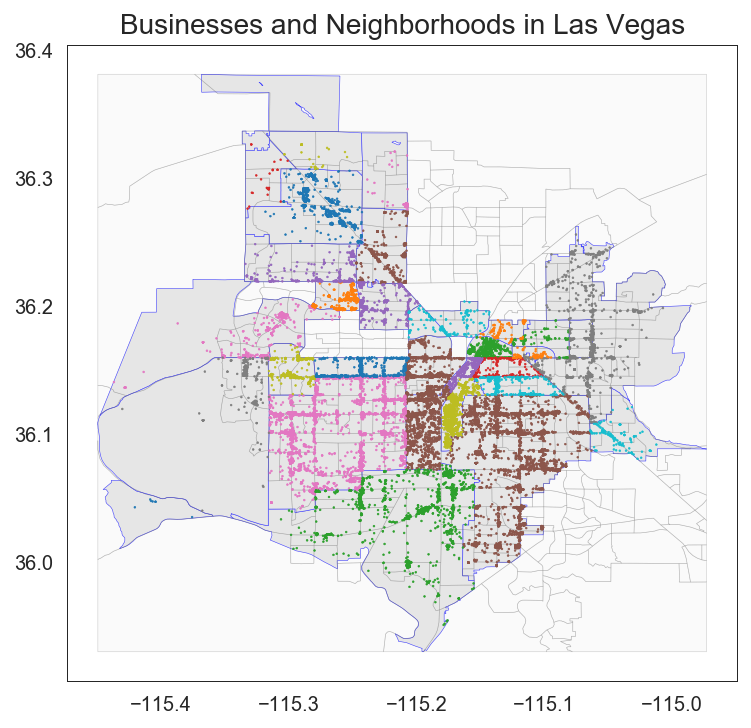
\includegraphics[width=0.5\textwidth]{las-vegas.png}
  \caption{Neighborhoods, census tracts, and businesses in Las Vegas. Polygons in darker shade are neighborhoods.}
  \label{vegas}
\end{figure}


After dropping businesses not in the top eight states and neighborhoods/census tracts without any businesses, we obtain 792 neighborhoods,  2,981 census tracts, and 115,522 businesses. Among the 115,522 businesses, 71,315 have neighborhood information. Table \ref{quartiles} displays the quartiles of business counts.

\begin{table}[htbp]
\caption{Quartiles of business counts}
\label{quartiles}
\centering
\begin{tabular}{lr|rrrrr}
\toprule
{} & n & min &  25\% &  50\% &  75\% &    max \\
\midrule
Neighborhood & 792 &  1 &   3 &  13 &  38 &  5454 \\
Census Tract & 2981 &  1 &   6 &  19 &  45 &  1767 \\
\bottomrule
\end{tabular}
\end{table}

For both geographic levels, at least half of the observations have less than 20 businesses. While one may argue they are residential areas and being residential is also one of the neighborhood characteristics, we still need at least a couple of businesses to detect \textit{business dynamics}.

We experimented different cutoff values to exclude neighborhoods with fewer businesses and decided that the minimal number of businesses being 10 was an appropriate threshold for making sure each neighborhood have enough businesses to aggregate measures from while without losing too many observations.

\section{Feature Extraction}

The features aggregated from the Yelp dataset are either proportion of businesses with a certain attribute, or basic statistics of some variables for all businesses located in a given area.

The features collected from census data are relatively straightforward and only needed minimal processing.

\subsection{Business Dynamics for Neighborhoods}

We can easily computer some basic features from the \texttt{business} table by creating a simple pivot table or calculating averages for groups. These features include the total number of businesses, number of businesses that are still open, average number of reviews per business, and average star ratings, as displayed in Table \ref{city-biz-table}.

We also included the proportion of businesses in the top categories and businesses having values for a few selected attributes as features. 

\subsubsection{Business categories}

The business categories of Yelp are hierarchical and a business may belong to multiple categories. We pick only a few most common top-level categories and a few second-level categories in \texttt{Restaurants} and \texttt{Food} that we deem descriptive for a neighborhood as our features. Fig. \ref{categories} displays the number of businesses in the top-level categories for the reduced dataset.

\begin{figure}[h]
  \hspace{-.5em}
    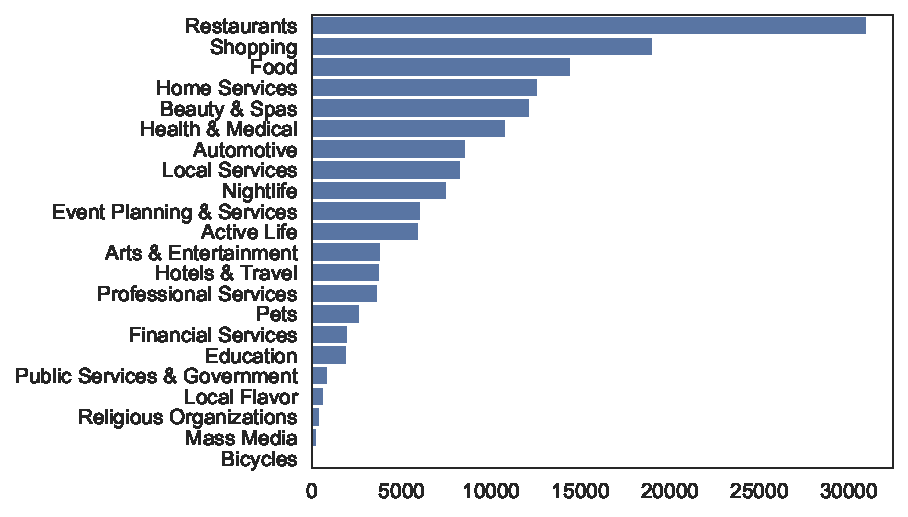
\includegraphics[width=0.493\textwidth]{categories}
  \caption{Number of businesses in top-level categories}
  \label{categories}
\end{figure}

The categories we added to the features are: Restaurants, Shopping, Food, Home Services, Beauty \& Spas, Health \& Medical, Automotive, Local Services, Shopping, Nightlife, Hotels \& Travel and Coffee \& Tea (a secondary category in Food). The first nine are the top nine categories with most businesses; ``Hotels \& Travel'' is added because it may be representative to touristic areas; ``Coffee \& Tea`` is added as it generally represents a laid-back lifestyle.

\subsubsection{Business attributes}

Attributes are metadata about whether a business provides certain types of services. There are in total 39 attributes, eight of them are restaurants-only, and others are mostly related to food and drink outlets such as cafes and bars. Because of the nature of these attributes, a majority of the non-eating-related businesses do not have a value set for most attributes. But for categories that are relevant, the fullness of the attributes are indeed satisfiable (Fig. \ref{attributes}).

\begin{figure}[h]
  \hspace{-.5em}
    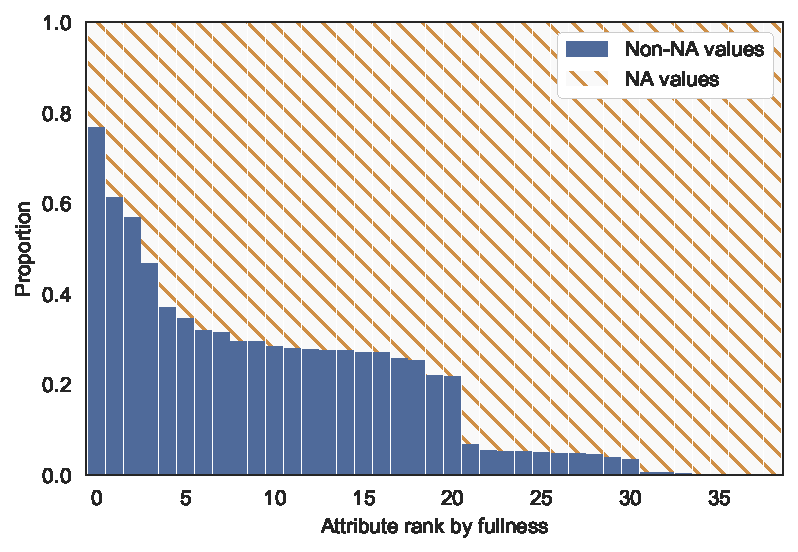
\includegraphics[width=0.48\textwidth]{attributes}
  \caption{Fullness of business attributes. The plateau between attribute 5 and 20 indicates attributes unique to certain categories have relatively unvaried fullness.}
  \label{attributes}
\end{figure}

The attributes we chose to include in the feature matrix are:
\begin{enumerate}
	\item \textit{DressFormal}: whether a restaurant has a formal dress code.
	\item \textit{RestaurantsPriceRange2}: the price range from scale 1 (cheapest) to 4 (most expensive).
	\item \textit{Alcohol}: whether the establishment offers alcohol beverages.
	\item \textit{RestaurantsTakeOut}: whether the restaurant accepts takeout orders.
\end{enumerate}

They were all calculated as proportions of true values among non-NA values.

\subsection{Advanced Features}

\subsubsection{Open hours}

Using the open hours information, we created three variables for each business: number of open hours  in the weekdays, number of open hours in the weekends, and whether the business is open at night (after 8 pm).

\subsubsection{Business density} We could use the land areas to calculate business density, but since the sizes of neighborhoods and census tracts vary a lot, we opt for a more representative measurement---Distance Band weights. We calculated the number of neighboring businesses within a radius of 2 kilometers for each business, then for each neighborhood, its business density measurement is just the average number of neighboring businesses in 2km for all businesses within it.

\subsection{Data Audit and Imputation}

\subsubsection{Yelp }
We have limited our aggregations to geographic units with at least 10 businesses, but since some attributes are only present for food establishments, there are still a few NA's in the aggregated measurements---i.e., some neighborhood may not have a variable for how many restaurants require guests to dress formally, because there are no restaurants in it at all. We imputed all missing values with the median of corresponding variables.

In the end, for the Zillow neighborhood level, we built a $442 \times 24$ feature matrix out of the Yelp data, representing the business dynamics of neighborhoods.

The distribution of major variables in this feature matrix are shown in Fig. \ref{nbh-histo}. It can be seen that business count (\texttt{n\_biz}) is the most skewed variables---even after we filtered out neighborhoods with few businesses, the majority of the neighborhoods still have only less than 100 businesses, while a handful of large neighborhoods can have as many as 5,400+ businesses. Most other variables follow normal distribution, except for count variables (\texttt{n\_biz\_in\_2km}, \texttt{review\_count}) and those for the least common categories (\texttt{HomeServices}).

\begin{figure}[h]
  \hspace{-.5em}
    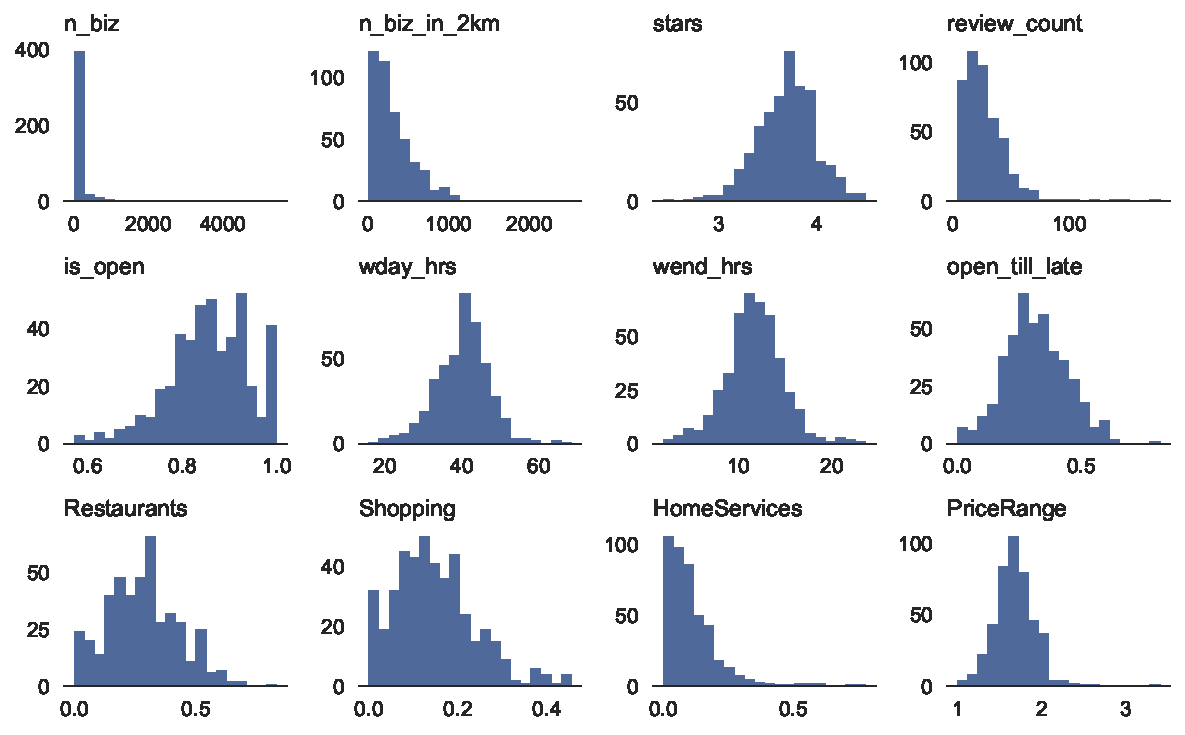
\includegraphics[width=0.5\textwidth]{nbh-histo}
  \caption{Histogram of major variables for business dynamics aggregated at the Zillow neighborhood level}
  \label{nbh-histo}
\end{figure}

We then used Pearson's correlation coefficient to test the correlations between variables. As shown in Fig. \ref{nbh-corr}, the most independent variable is \texttt{is\_open}, the ratio of businesses that are still open. Both business density and review count are positively correlated with business count. Weekend open hours and open till late positively correlate with the proportion of restaurants, shopping, and food establishments, but negatively correlate with the proportion of home services and other businesses, which should not be to anyone's surprise. We see also where there are more restaurants, there are less home services. Arts and Entertainment businesses are more likely to be located in where there are more nightlife and businesses requiring formal dressing.

\begin{figure}[h]
  \hspace{-.5em}
    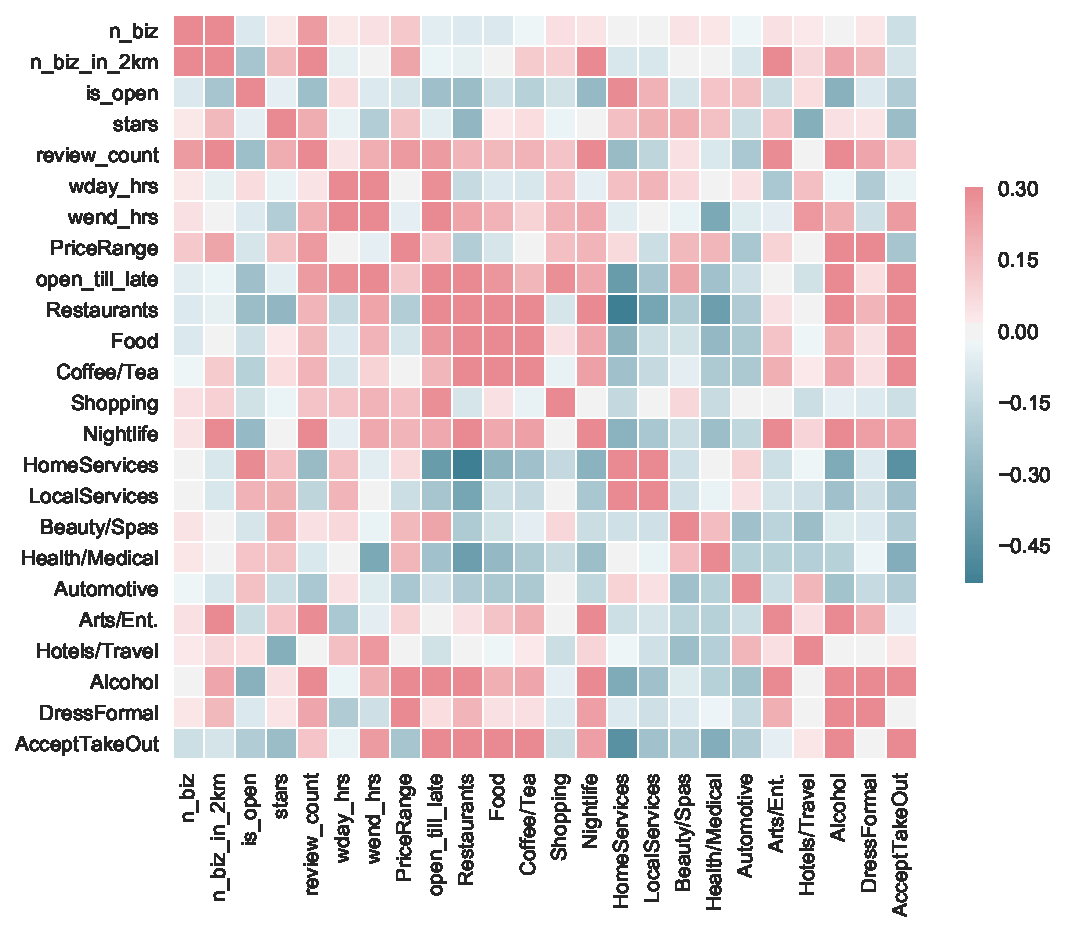
\includegraphics[width=0.5\textwidth]{nbh-corr}
  \caption{Correlation heatmap for all features aggregated at the census tract level}
  \label{nbh-corr}
\end{figure}

\section{Clustering}

We mainly tested two clustering algorithms---K-Means, GMM---on the Yelp dataset at both the Zillow neighborhood and census tract level, and evaluated how the choice of aggregation level, variables, preprocessing steps and clustering methods may impact the outcome.

We then ran clustering algorithms on the census data and identified clusters based on population characteristics and socioeconomic metrics. We used the clusters at this step as a reference for evaluating the clustering of neighborhoods by business dynamics.

\subsection{Business Dynamics by Zillow Neighborhood}

\subsubsection{K-Means clustering without feature scaling}

We first applied K-Means on the raw business dynamics features aggregated at the Zillow neighborhood level without any preprocessing. The elbow method indicates the optimal cluster number is 4 (Fig. \ref{nbh-kmeans}).

\begin{figure}[h]
  \hspace{-.5em}
    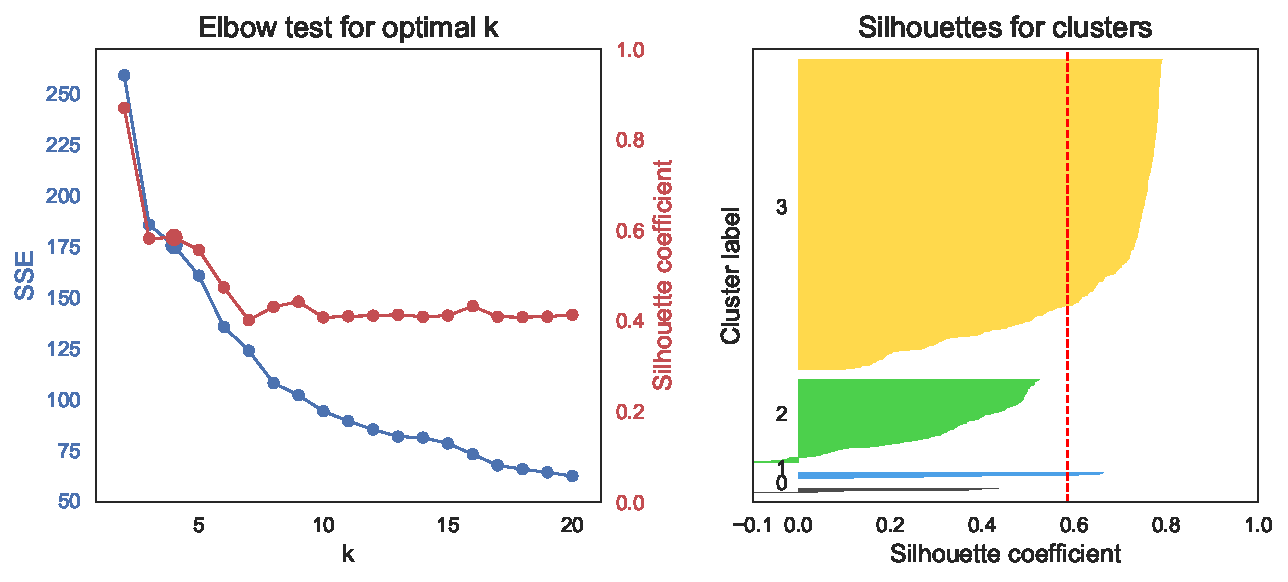
\includegraphics[width=0.5\textwidth]{nbh-kmeans}
  \caption{K-Means clustering for neighborhoods. The larger markers in the left plot indicate optimal $k$, the red line in the right plot indicates the silhouette coefficient with the optimal $k$.}
  \label{nbh-kmeans}
\end{figure}

The highly skewed variable \texttt{n\_biz} (number of businesses in a neighborhood) dominated the clustering process and made the sizes of clusters extremely uneven. The fact that it has far larger scale than other variables also made it harder to account for other variables. We could see from the cluster labels that the smaller clusters contained only neighborhoods with a very high amount of businesses (Table \ref{nbh-centroids}). In fact, if we let $k = 2$, the average silhouette score would jump from $0.58$ ($k = 4$) to $0.87$, indicating an even better separating of neighborhoods. While it is not technically wrong that neighborhoods with many businesses are vastly different from others, we would still want to uncover more nuanced patterns.

This led us to investigate feature scaling techniques.

\begin{table*}[htbp]
\caption{K-Means centroids of neighborhoods without feature scaling *}
\label{nbh-centroids}

\begin{tabular}{lrrrrrrrrr}
\toprule
{} &    n &    n\_biz &  n\_biz\_in\_2km &  is\_open &  stars &  review\_count &  wday\_hrs &  wend\_hrs &  PriceRange \\
\midrule
0 &    6 &  3600.67 &       1096.05 &     0.81 &   3.80 &         66.53 &     41.67 &     12.72 &        1.93 \\
1 &    7 &  1713.86 &        485.48 &     0.84 &   3.70 &         37.31 &     40.10 &     11.60 &        1.66 \\
2 &   91 &   188.30 &        710.38 &     0.83 &   3.76 &         38.47 &     39.11 &     11.67 &        1.72 \\
3 &  338 &    57.40 &        201.81 &     0.86 &   3.67 &         23.61 &     40.46 &     11.75 &        1.66 \\
\midrule
{} &    n &  open\_till\_late &  Rest &  Food &  Coffee/Tea &  Shopping &  Nightlife &  HomeServices &  LocalServices \\
\midrule
0 &    6 &            0.29 &  0.23 &  0.11 &        0.02 &      0.17 &       0.09 &          0.10 &           0.06 \\
1 &    7 &            0.26 &  0.22 &  0.11 &        0.02 &      0.17 &       0.05 &          0.14 &           0.09 \\
2 &   91 &            0.30 &  0.29 &  0.15 &        0.03 &      0.15 &       0.10 &          0.11 &           0.07 \\
3 &  338 &            0.32 &  0.28 &  0.14 &        0.02 &      0.15 &       0.05 &          0.11 &           0.08 \\
\midrule
{} &    n &  Beauty/Spas &  Health/Medic &  Automotive &  Arts/Ent. &  Hotels/Travel &  Alcohol &  DressFormal &  AcceptTakeOut \\
\midrule
0 &    6 &         0.13 &          0.11 &        0.05 &       0.05 &           0.04 &     0.16 &         0.01 &           0.22 \\
1 &    7 &         0.09 &          0.09 &        0.09 &       0.03 &           0.04 &     0.10 &         0.00 &           0.23 \\
2 &   91 &         0.09 &          0.07 &        0.07 &       0.06 &           0.03 &     0.16 &         0.01 &           0.30 \\
3 &  338 &         0.10 &          0.09 &        0.08 &       0.02 &           0.03 &     0.12 &         0.00 &           0.31 \\
\bottomrule
\end{tabular}

\vspace{1em}
\small{* The first column represents cluster label, the second column is the number of neighborhoods in the cluster}

\end{table*}


\subsubsection{K-Means clustering after feature scaling}

Feature scaling puts all variables at the same scale, so the effects of them could be compared more fairly. We tested three scaling techniques: \textit{standardized normal distribution} removes the mean of a variable and divide each sample with the variance; \textit{min-max scaler} and \textit{quantile transformation} put variables at the $[0, 1]$ range.

All of them reduced the silhouettes significantly. Since there were not clear elbow in the SSE test, we kept the number of clusters at  $4$. The silhouettes dropped from $0.58$ to the $0.10$ range, with standardized normal distribution showing slightly better performance (Fig. \ref{nbh-kmeans-standardized}).

\begin{figure}[h]
  \hspace{-.5em}
    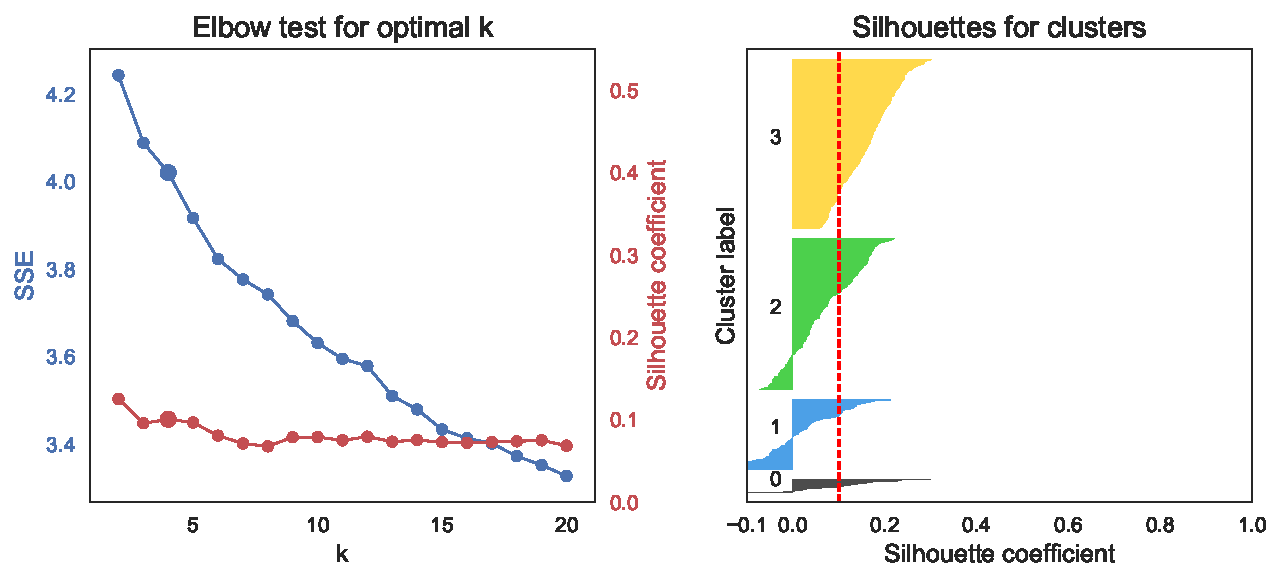
\includegraphics[width=0.5\textwidth]{nbh-kmeans-standardized}
  \caption{K-Means clustering after standardization. The average silhouette for $k = 4$ is $0.1006$. Scaling with the min-max scaler and quantile transformation produced silhouettes $0.0965$ and $0.0988$ respectively.}
  \label{nbh-kmeans-standardized}
\end{figure}

Dimension reduction with Principal Component Analysis (PCA) confirmed that standardization on all variables made it harder to tell different neighborhoods apart. In Fig. \ref{nbh-pca}, features were reduced to two principal components. To calculate the covariance for PCA, features must be standardized. The difference between the graph on the left and that on the right is that individual samples for the right were converted to unit form before applying PCA. We could see an obvious cluster on the right side because sample normalization captured the skewness of the count variables before the standardization.

\begin{figure}[h]
  \hspace{-.5em}
    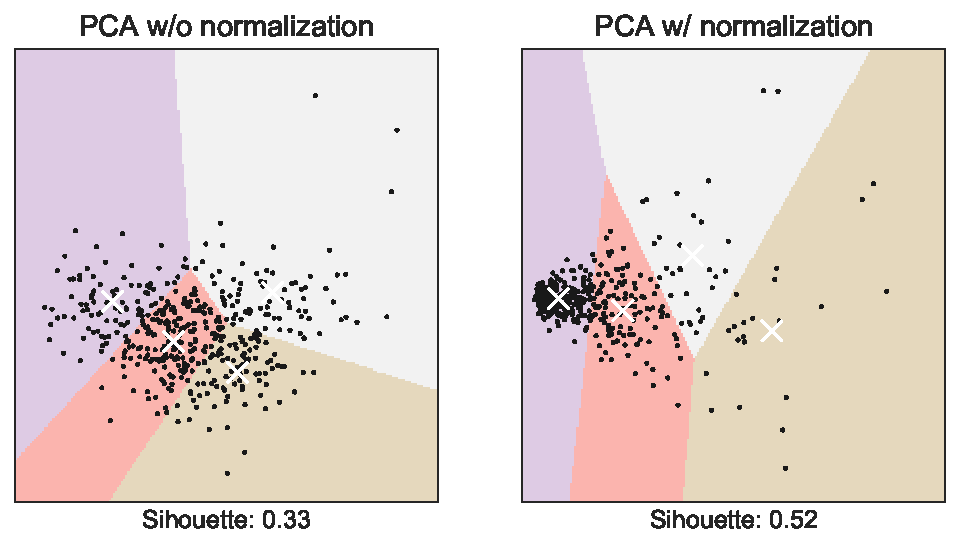
\includegraphics[width=0.5\textwidth]{nbh-pca}
  \caption{K-Means clusters for PCA reduced features. 24 variables were reduced to 2 components. Normalized data preserved the skewness of the count variables, hence showing a more obvious cluster.}
  \label{nbh-pca}
\end{figure}

\subsubsection{Transform count data to log values}

Another popular technique in handling highly skewed count data is to apply log transformation so it may result in some sort of linear relationship. However, applying log transformation on our aggregated measurements did not help the clustering.

When we applied log transformation to either \texttt{n\_biz} or \texttt{n\_biz\_in\_2km} (business density), or both, the effect was very similar to simply removing the variables, regardless whether we applied standardization afterwards or not.

\subsubsection{Weighted feature scaling}

In addition to the unsatisfactory result, one of the problems with standardization on all variables is that it makes the results harder to interpret and interpretability is the often the key to data analysis for social science. Furthermore, most detrimentally, this approach considers all variables of the same importance, which is certainly not the case for the purpose of our study.

Therefore we took a more mindful approach and introduced weighted feature scaling to make sure models are resilient to outliers while remaining interpretable.

Based on the variable types, after multiple trials, we assigned following weights to the variables.

\begin{enumerate}
	\item \textbf{n\_biz}: $0.01$. Each unit now represents 100 businesses.
	\item \textbf{Coffee/Tea, Nightlife, DressFormal, Arts/Ent.}: $1000$. special business types implying the affluence of a neighborhood.
	\item \textbf{stars}: $20$. Yelp ratings of the businesses. Multiple by $20$ to boost importance, effectively convert the scale of 1 to 5 stars to a 100-point system.
	\item \textbf{wday\_hrs, wend\_hrs}: $10$. Number of open hours of businesses. Multiply by $10$ to boost importance.
	\item \textbf{Other proportional variables}: $100$. Effectively scales percentages from $[0, 1]$ range to $[0, 100]$ range.
\end{enumerate}

Fig. \ref{nbh-kmeans-weighted} shows the clustering outcome for weighted features. Although $k = 6$ seemed more like the elbow for optimal $k$, we kept the $k$ at $4$ for ease of interpretation and evaluation. Table \ref{nbh-centroids-weighted} shows the updated centroids. The neighborhoods were reasonably separated, while business density was still the major factor (as we wanted it to be), we could see arts, nightlife, coffee places, and fine dining (\texttt{DressFormal}) are more likely to concentrate at high-density areas.

\begin{figure}[h]
  \hspace{-.5em}
    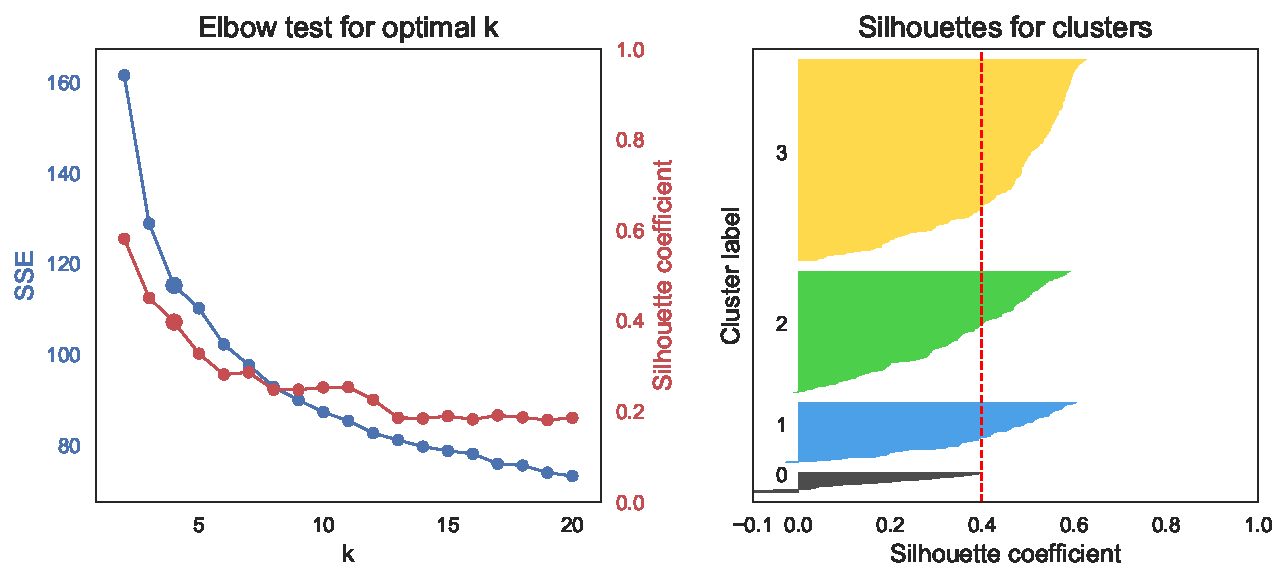
\includegraphics[width=0.5\textwidth]{nbh-kmeans-weighted}
  \caption{K-Means clusters for features scaled with weights.}
  \label{nbh-kmeans-weighted}
\end{figure}

\begin{table*}[htbp]
\caption{K-Means centroids of neighborhoods with weighted feature scaling}
\label{nbh-centroids-weighted}

\begin{tabular}{lrrrrrrrrr}
\toprule
{} &    n &  n\_biz &  n\_biz\_in\_2km &  is\_open &  stars &  review\_count &  wday\_hrs &  wend\_hrs &  PriceRange \\
\midrule
1 &   22 &   8.33 &       1113.21 &    80.90 &  73.61 &         46.28 &    373.34 &    117.47 &      183.35 \\
3 &   67 &   3.00 &        652.09 &    83.25 &  75.54 &         39.04 &    398.86 &    118.18 &      170.52 \\
2 &  132 &   1.52 &        358.62 &    84.25 &  75.25 &         30.00 &    400.48 &    112.58 &      170.15 \\
0 &  221 &   0.52 &        123.59 &    87.55 &  72.52 &         20.57 &    406.50 &    120.15 &      163.27 \\
\midrule
{} &    n &  open\_till\_late &   Rest &   Food &  Coffee/Tea &  Shopping &  Nightlife &  HomeServices &  LocalServices \\
\midrule
1 &   22 &           28.61 &  34.29 &  14.67 &       34.56 &     12.71 &     170.96 &          6.98 &           6.42 \\
3 &   67 &           30.85 &  27.80 &  15.33 &       32.53 &     15.23 &      82.46 &         11.59 &           6.88 \\
2 &  132 &           31.03 &  23.77 &  12.60 &       25.75 &     16.49 &      48.19 &         10.68 &           7.97 \\
0 &  221 &           32.18 &  30.70 &  14.78 &       24.41 &     13.55 &      47.82 &         11.33 &           7.98 \\
\midrule
{} &    n &  Beauty/Spas &  Health/Medic &  Automotive &  Arts/Ent. &  Hotels/Travel &  Alcohol &  DressFormal &  AcceptTakeOut \\
\midrule
1 &   22 &         6.89 &          4.96 &        4.41 &      87.69 &           5.27 &    24.01 &        22.00 &          31.69 \\
3 &   67 &         9.30 &          7.64 &        7.66 &      50.82 &           2.81 &    14.26 &         6.00 &          29.20 \\
2 &  132 &        11.53 &         11.93 &        6.68 &      28.69 &           2.45 &    11.87 &         6.39 &          26.40 \\
0 &  221 &         9.02 &          7.74 &        7.96 &      20.52 &           2.88 &    11.72 &         2.60 &          33.06 \\
\bottomrule
\end{tabular}

\end{table*}


\subsubsection{GMM clustering}

It is evident that at least for Zillow neighborhoods, the variables we built intrinsically do not have a strong clustering effect. Gaussian Mixture Model (GMM) experienced even more difficulties in separating neighborhoods apart.

Without normalization or PCA, GMM was not even able to converge within 100 iterations. After testing various combinations of preprocessing steps and variable choices, we found that PCA reduction without normalization and with the covariance type \texttt{full} (each component has its own general covariance matrix) produces the best result. Fig. \ref{nbh-gmm-bic} and Fig. \ref{nbh-gmm} demonstrates how this model was selected.

Weighted feature scaling did not improve results for GMM clustering.

\begin{figure}[h]
  \centering
  \hspace{-.5em}
    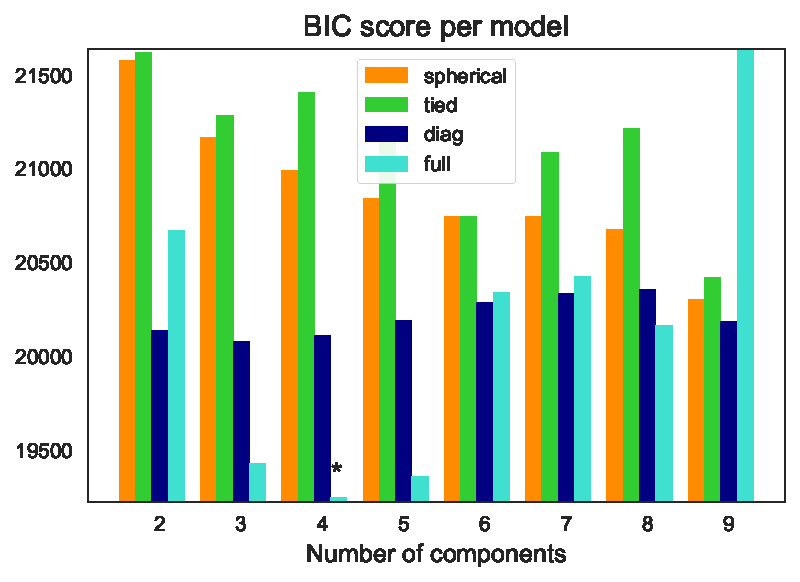
\includegraphics[width=0.48\textwidth]{nbh-gmm-bic}
  \caption{GMM model selection with BIC score. Lower score is preferred. This graph shows that the best model is when clustering with \textit{full} covariance matrix and aiming for $4$ Gaussian distribution components.}
  \label{nbh-gmm-bic}
\end{figure}

\begin{figure}[h]
  \hspace{-.5em}
    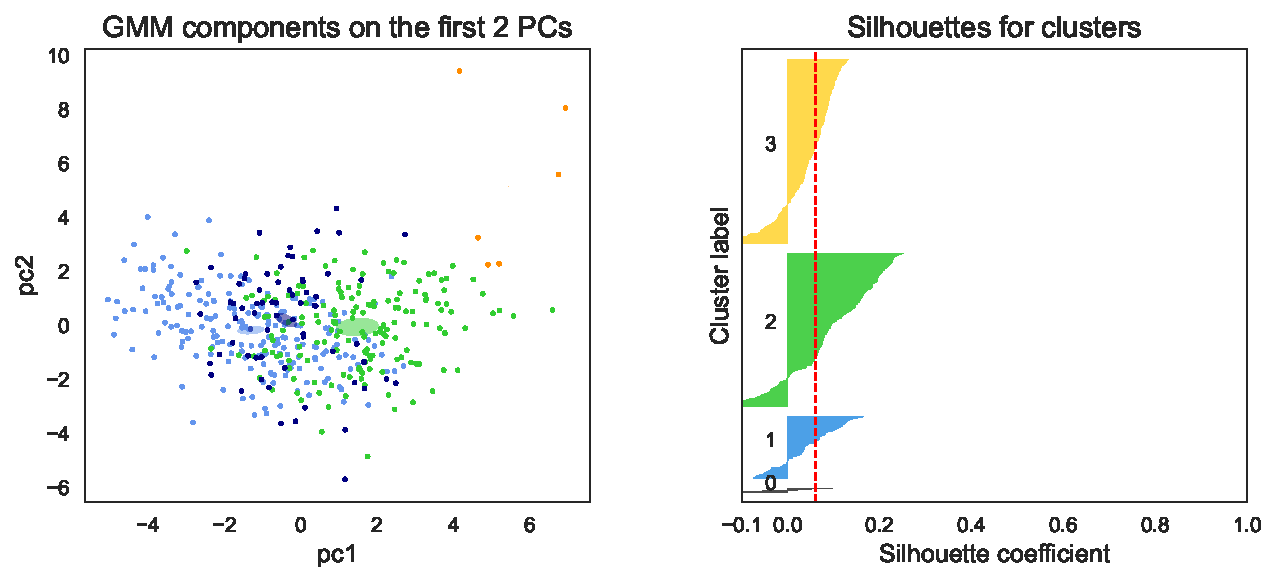
\includegraphics[width=0.5\textwidth]{nbh-gmm}
  \caption{GMM best model outcome after PCA reduction. The plot on the left visualizes the first principal components and the predicted cluster labels. The plot on the right shows the silhouette coefficients. Because of the overlap of GMM components, the cluster predictions were not able to separate neighborhoods apart.}
  \label{nbh-gmm}
\end{figure}

\subsection{Business Dynamics by Census Tract}

In the next step, we applied the same clustering methods on the same set of features aggregated at the census tract level. Even though we had four times more observations ($1987 \times 24$ v.s. $442 \times 24$), the outcome was unsurprisingly very similar---after all, census tracts are just smaller neighborhoods. 

The results showed the same patterns: business density continued to dominate; businesses in high-density areas receive more reviews; when count data were removed, length of work hours became the strongest differentiator.

We ran this additional clustering test only to be able to evaluate clustering by business dynamics with the census data.

\subsection{Neighborhood Characteristics by Census Tract}

To answer the question how patterns of business dynamics associate with neighborhood characteristics, we ran clustering with the census data, too.

As mentioned, most of the census variables are of a "variable group", i.e., a set of variables describing each subgroup of the same population attribute. For example, there are 11 variables for age groups. These variables are intrinsically highly correlated with each other. To abate such multicollinearity, we employed PCA again to reduce the dimensionality of the census variables. The 71 census variables were easily reduced to 26 components, while explaining 91\% of the variance.

GMM clustering worked moderately better with the census data. After feature reduction, the model with covariance type \texttt{full} and number of components $k = 4$ achieved a silhouette of $0.16$, comparing to that of $0.14$ by K-Means and, $0.01$ for clustering the Yelp data.

\subsection{Evaluation of the Clusters}

After clustering two datasets separately, we used confusion matrix and purity score to evaluate the goodness of the clusters. We compared the overlap of two sets of clusters: clustering by Yelp data and clustering by census data, both at the census tract level. Additional steps were taken to make sure they have the same number of observations and represent the same set of census tracts.

Clusters obtained from census data were considered the ``ground truth'', even though it was also obtained from algorithms. Table \ref{confusion-1} shows the confusion matrix for comparing the clusters obtained from two data sources. The columns represent cluster labels for census tracts obtained from running GMM on PCA-reduced census data; the rows represent cluster labels based on K-Means and weight-scaled business dynamics data.

We noticed that all purity scores for each row were calculated based on the overlap between the Yelp data clusters and the largest census data cluster. Basically the largest cluster by census data encompassed the majority of the census tracts in all clusters by business dynamics. This is certainly not desired. We tested different combinations of preprocessing steps and model choices. Unfortunately, the results were more or less the same.

It seemed impossible to use clustering methods to explain business dynamics with census data. After all, there were no practical clusters in both data sources to begin with (simply separating a few high-density neighborhoods was not particularly useful).

\begin{table}[h]
\centering
\caption{Confusion matrix for the overlaps of clusters}
\label{confusion-1}
\bgroup
\def\arraystretch{1.5}
\begin{tabular}{lrrrr|r|r}
\toprule
{} &    0 &     1 &   2 &    3 &  Total &  Purity \\
\hline
0     &  360 &   617 &  12 &  114 &   1103 &  0.5594 \\
1     &   14 &    29 &   1 &    1 &     45 &  0.6444 \\
2     &  191 &   298 &  10 &   53 &    552 &  0.5399 \\
3     &   76 &   154 &  16 &   23 &    269 &  0.5725 \\
\hline
Total &  641 &  1098 &  39 &  191 &   1969 &  0.5576 \\
\bottomrule
\end{tabular}
\egroup
\end{table}

\subsection{Suprivised Variable Selection}

In our last attempt to optimize the models, since we already knew business density was the deciding factor among the features extracted from Yelp data, we wanted to see whether choosing only  census variables that have a strong correlation with business density would improve the clustering outcome.

We used RandomForest to select the important variables in terms of predicting business density. The top 4 variables were: proportion of households that are nonfamily (people who live alone or with nonrelatives only); proportion of people who are born in the sate they live; population density; GINI coefficient for income inequality.

Using these variables only, we tested the clustering algorithms again and GMM model found some interesting pattern. As shown in Fig. \ref{aci-rf-gmm}, there were clear clusters at least for the first two variables. For a neighborhood less likely to have nonfamily households, it either has a lot of residents born in the sate, or have much fewer. Few neighborhoods were somewhere in between.

On the other hand, we did see a slight improvement in purity scores and the sizes of clusters also became more even (Table \ref{confusion-2}).


\begin{figure}[ht]
  \centering
  \hspace{-.5em}
    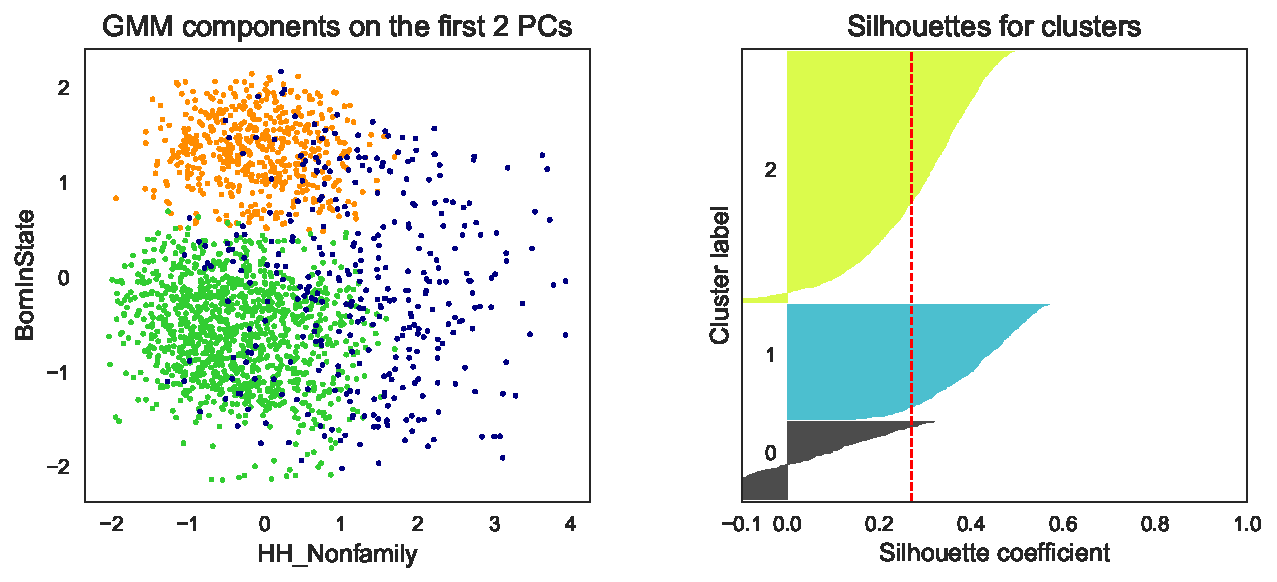
\includegraphics[width=0.48\textwidth]{aci-rf-gmm}
  \caption{GMM and selected census variables.}
  \label{aci-rf-gmm}
\end{figure}

\begin{table}[ht]
\centering
\caption{Confusion matrix for cluster overlaps by RandomForest selected variables}
\label{confusion-2}

\bgroup
\def\arraystretch{1.5}
\begin{tabular}{lrrrr|r|r}
\toprule
{} &   0 &    1 &    2 &    3 &  Total &  Purity \\
\hline
0     &  12 &  398 &  191 &   33 &    634 &  0.6278 \\
1     &  25 &   84 &   75 &  298 &    482 &  0.6183 \\
2     &  34 &   29 &  114 &   15 &    192 &  0.5938 \\
3     &  20 &  339 &  142 &  160 &    661 &  0.5129 \\
\hline
Total &  91 &  850 &  522 &  506 &   1969 &  0.5835 \\
\bottomrule
\end{tabular}
\egroup

\end{table}


\section{Results and discussion}

In this paper, we used reverse geocoding to handle missing neighborhood information in the Yelp data, built metrics for describing business dynamics of neighborhoods, then employed various data mining techniques and clustering algorithms to analyze the explainability of neighborhood characteristics to business dynamics.

We found that business dynamics of neighborhoods were mainly defined by business density and high-density areas also tend to attract more user reviews and contain more arts/entertainment, and nightlife businesses. Other than the density-related variables, other variables we have selected were not able to demonstrate high explainability in K-Means and GMM clustering.

Data normalization helped us uncover more nuanced patterns; PCA was useful in cluster visualization; weighted feature scaling helped us build more interpretable models. Mindful selection of variables and reducing noises was also very important for clustering processes.

 We assumed clustering by neighborhood characteristics as the ground truth, but those variables had feeble clustering effect themselves. After identifying variables most relevant to business density, we saw only minor improvement in clustering performance.

The difficulty in using clustering algorithms to separate neighborhoods apart by either business related metrics or population characteristics confirms that there are no two neighborhoods are alike. They may be similar in some measurements, but they must have differences in others.

In future work, to understand the interactions between businesses and neighborhoods, we shall take a more mindful approach and select only variables representing a specific aspect of urban living and social fabric. For example, we can focus on the cultural vibrancy of a neighborhood, using proportion of arts/entertainment businesses, and topic modeling from user reviews or social media posts as measurements. We may also want to make subgroups of neighborhoods based on their sizes, business counts, or whether or not located in or adjacent to urban centers.


\printbibliography[title={References}]


\appendix[Full list of census variables]

\footnotesize{\begin{lstlisting}
Female                      Male                      
AgeU5                       Age517                    
Age1824                     Age2534                   
Age3544                     Age4554                   
Age5559                     Age6061                   
Age6264                     Age6574                   
Age75P                      BornInState               
BornInOtherState            NativeBornOutOfUS         
ForeignBornNaturalized      ForeignBornNonCitizen     
White                       Black                     
Asian                       OtherRace                 
Hispanic                    TwoOrMore                 
MedHouseIncome              MedHousingCost            
MedHouseValue               MedRentAsIncomePct        
GINI                        SexRatio                  
Age6064                     AgeOld                    
Veteran                     HI_PrivateInsured         
HI_PublicInsured            HI_Insured                
NoSchool                    LessThanHS                
HSGrad                      SomeColl                  
Bach                        Master                    
Prof                        Doc                       
AtLeastBachelor             PopPerHousing             
VacentUnits                 OwnerOccupied             
RenterOccupied              BelowHalfPoverty          
BelowPoverty                BelowTwoPoverty           
AboveTwoPoverty             PubAssist                 
UnempRate                   ChildInNeed               
ChildInNeed_SingleParent    ChildInNeed_SingleMom     
ChildInNeed_Nonfamily       EthHet                    
HH_MarriedCouple            HH_SingleHead             
HH_MaleHead                 HH_FemaleHead             
HH_Nonfamily                HH_LiveAlone              
HH_NotAlone                 GrandHead                 
PopDen                                
\end{lstlisting}}

\end{document}